\section*{\centering \textit{\textbf{Appendix of VLA-Adapter}}}

\section{Setup Details of LIBERO Simulation Benchmarks}\label{Appendix_LIBERO_benchmark}

\renewcommand{\thefigure}{A\arabic{figure}}
\renewcommand{\theHfigure}{A\arabic{figure}}
\setcounter{figure}{0}

\renewcommand{\thetable}{A\arabic{table}}
\renewcommand{\theHtable}{A\arabic{table}}
\setcounter{table}{0}

The LIBERO benchmark \citep{LIBERO-2023} comprises four distinct task suites: LIBERO-Spatial, LIBERO-Object, LIBERO-Goal, and LIBERO-100. The first three suites each contain 10 tasks, and LIBERO-100 contains 90 short-term tasks (LIBERO-90) and 10 long-horizon tasks (LIBERO-Long). The strategy for each task depends solely on the current instructions provided. Each task is repeated multiple times (50 repetitions in this paper) to obtain the average success rate for each subtask. The examples and the instructions in the LIBERO benchmark are shown in Figure \ref{Figure_LIBERO}.

\begin{figure}[!htbp]
	\centering
	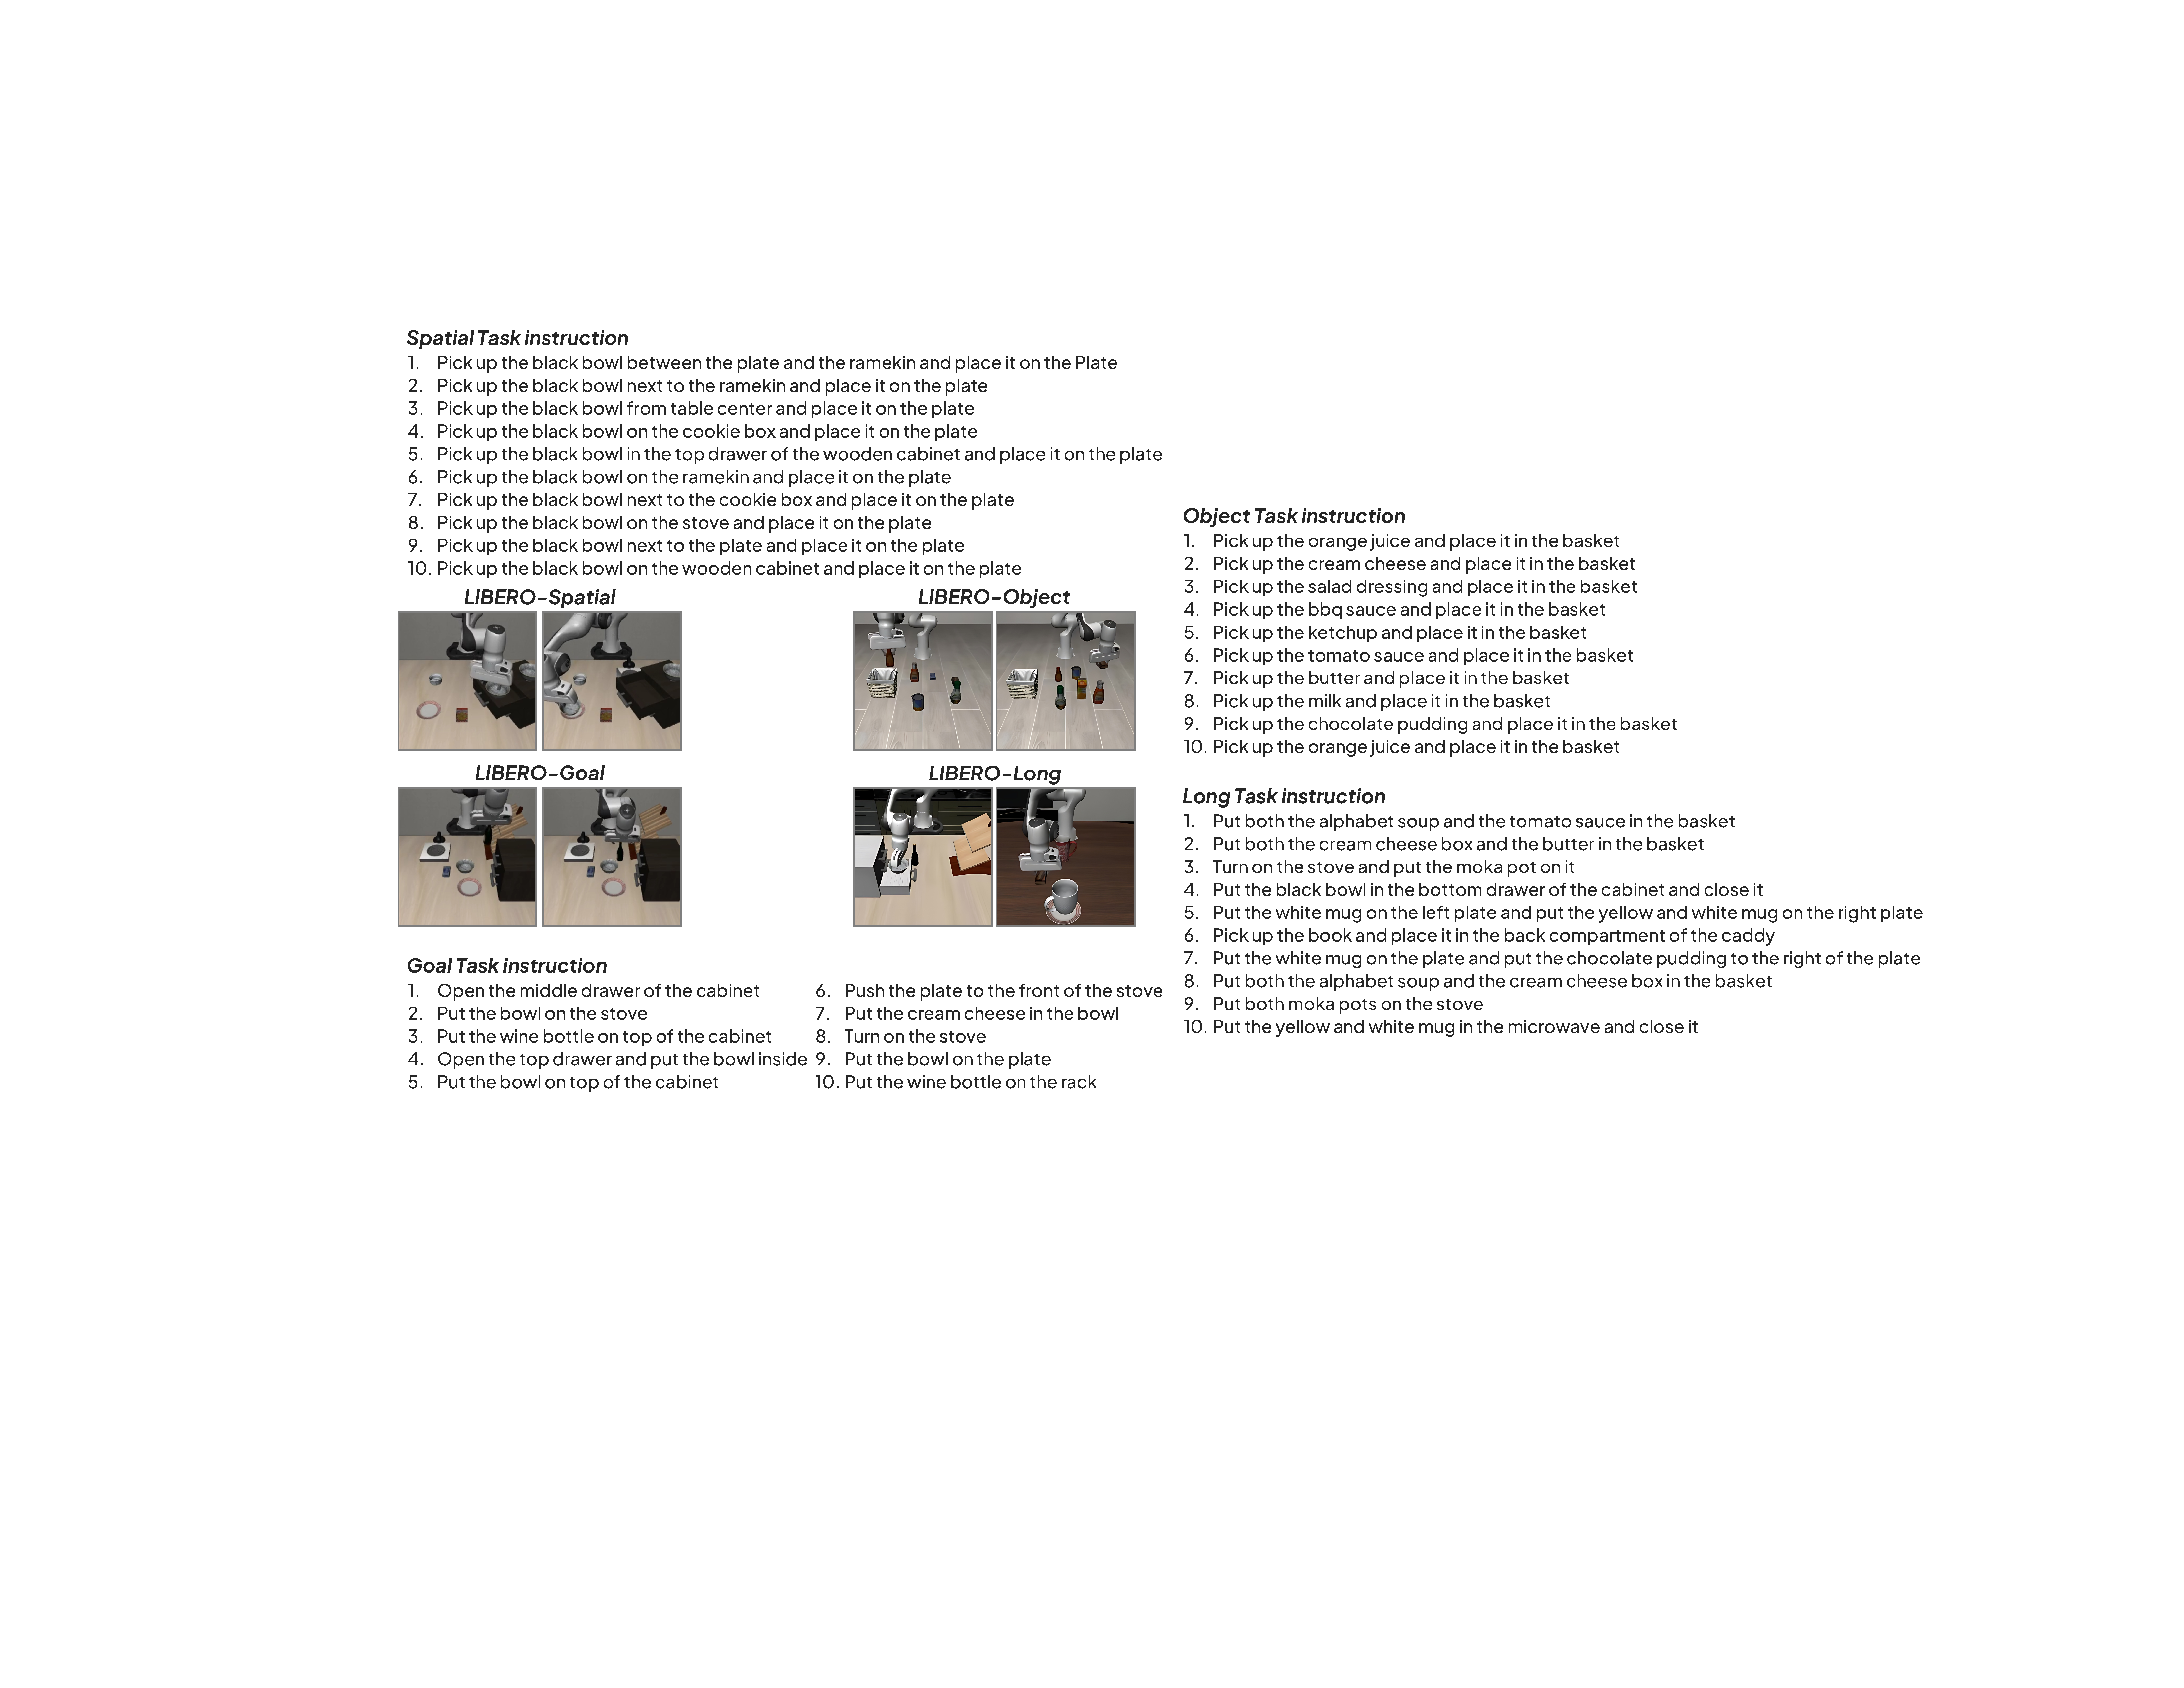
\includegraphics[width=0.99\textwidth]{Figures/Appendix-LIBERO.pdf}
	\caption{The examples and the task instructions on the LIBERO benchmark.}\label{Figure_LIBERO}
\end{figure}

In the LIBERO benchmark, we use third-person images (resolution 224$\times$224$\times$3, RGB) and wrist images (resolution 224$\times$224$\times$3, RGB) as visual input. The task instruction is first constructed as a prompt in a specific format: ``\texttt{In: What action should the robot take to {instruction.lower()}?\textbackslash nOut:}", and then input into the VLM module together with the image information. Its output is a 7-dimensional action vector, which is used to control the 7-DOF Franka Emika Panda simulated robot arm to perform the corresponding action sequence.

\vspace{3ex}

\section{DiT-Based Policy Network}\label{Appendix_DiT}
\renewcommand{\thefigure}{B\arabic{figure}}
\renewcommand{\theHfigure}{B\arabic{figure}}
\setcounter{figure}{0}

\renewcommand{\thetable}{B\arabic{table}}
\renewcommand{\theHtable}{B\arabic{table}}
\setcounter{table}{0}

\renewcommand{\theequation}{B-\arabic{equation}}
\renewcommand{\theHequation}{B-\arabic{equation}}
\setcounter{equation}{0}

\subsection{Overall Architecture}\label{Appendix_DiT_1} 

\begin{figure}[!htbp]
	\centering
	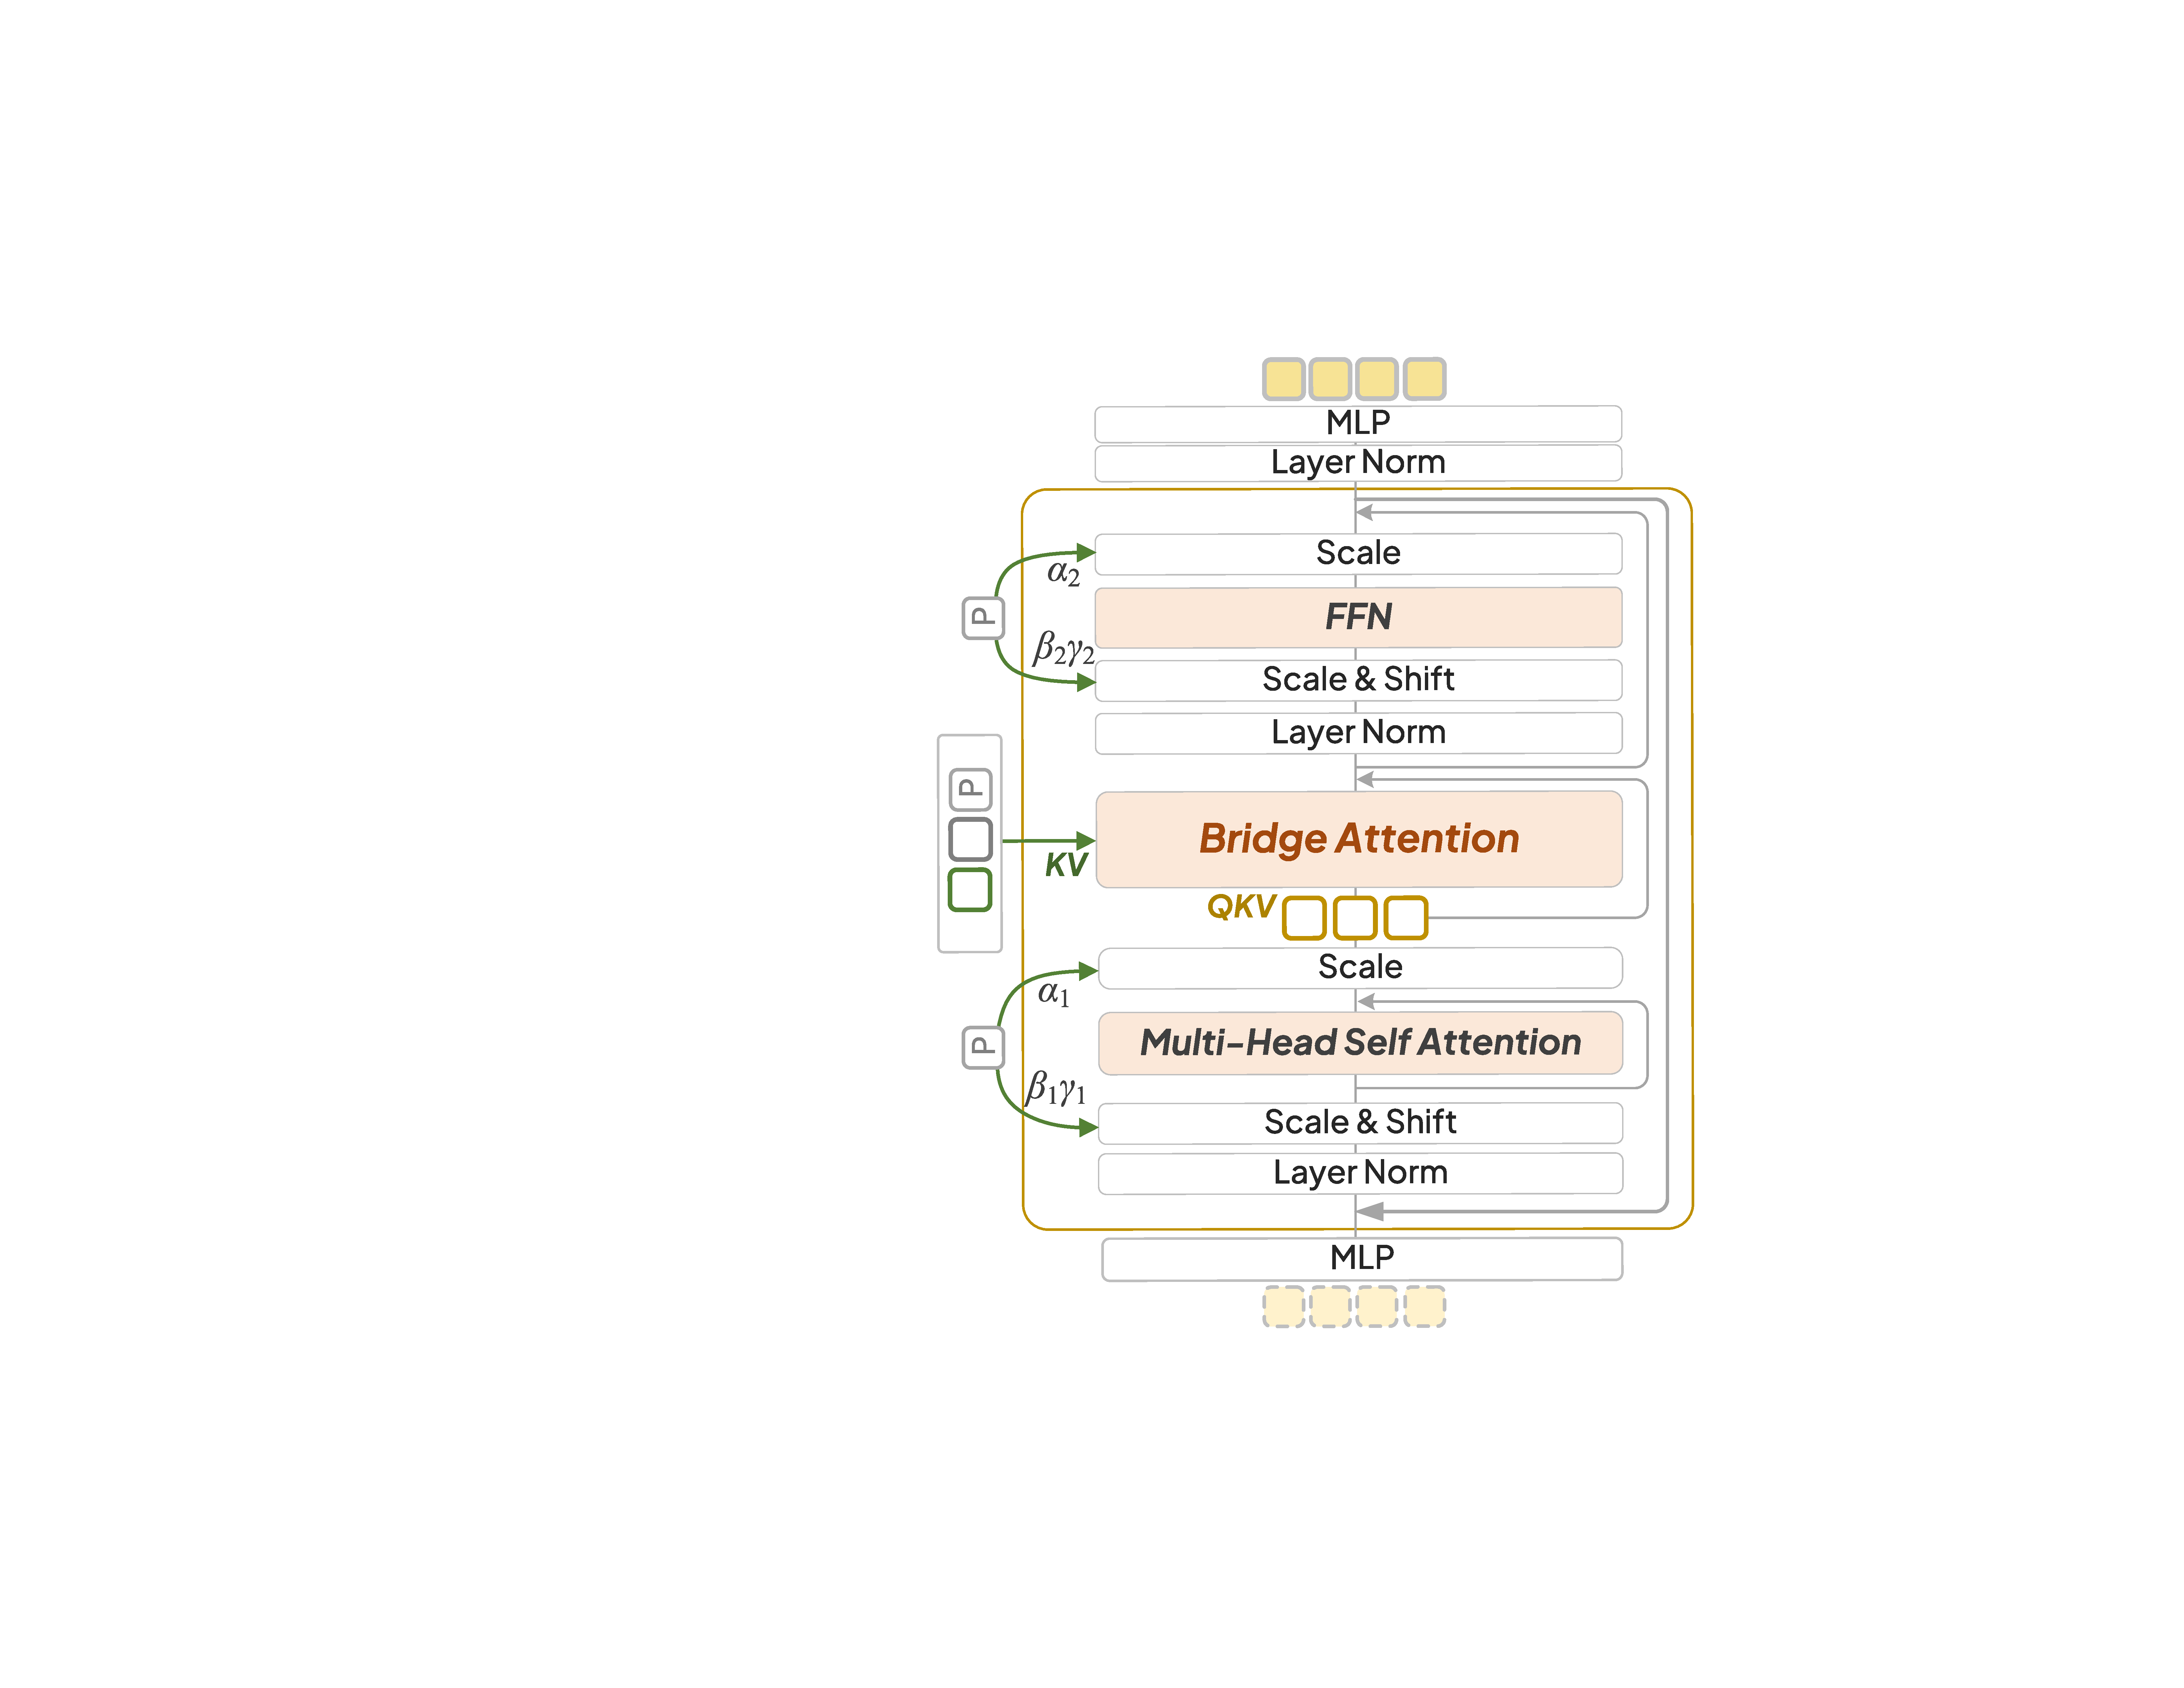
\includegraphics[width=0.45\textwidth]{Figures/DiT_policy.pdf}	
	\caption{The DiT-based policy network.}\label{Figure_DiT}
\end{figure}

This architecture is shown in Figure \ref{Figure_DiT}. It consists of $\tau$-DiT blocks, $1\leq\tau\leq M$. It has the same number of layers as VLM. Each DiT block consists of three components: conditional modulation, conditional attention, and a conditional feedforward network.
At timestep $t$, the input chunk to the first-DiT block, ${\bf A}^1_t$, is a noisy action sequence. Since the input contains random noise, to facilitate the transition from ``pure noise $\to$ fine-grained prediction", we adopt the AdaLN-Zero layer \citep{DiT-2023} to modulate the activation amplitude at each layer. The AdaLN-Zero consists of LayerNorm, modulation, and gated residual. Specifically, $C^{\mathcal{M}}_t$ will be obtained by $\mathcal{P}_t$ and $\mathcal{C}_t^{\mathcal{R}}$, i.e., $C^{\mathcal{M}}_t = \sigma'_1(\mathcal{C}_t^{\mathcal{R}}) + \sigma_0(\mathcal{P}_t)$. It is used to generate ``Scale" and ``Shift" vectors, which guide the activation direction of intermediate features and inject automatic modulation amplitude via gated residual control. After modulation, $\widetilde{\bf A}^1_t = \left[ \widetilde{\bf a}_t^1, \widetilde{\bf a}_{t+1}^1, \dots, \widetilde{\bf a}_{t+H-1}^1 \right]$ is obtained:

\begin{equation}\label{AppedixEq4}
\small
\widetilde {\bf A}_t^1  = {\bf{A}}_t^1  + {\alpha _\tau} \odot \varepsilon ({\gamma _\tau }{\mathop{\rm LN}\nolimits} ({\bf{A}}_t^1) + {\beta _\tau })= {\bf{A}}_t^1  + {\sigma' _2}(\mathcal{C}_t^\mathcal{M}) \odot \varepsilon ({\sigma'_1}^{(2)}(\mathcal{C}_t^\mathcal{M}){\mathop{\rm LN}\nolimits} ({\bf{A}}_t^1) + {\sigma'_1}^{(1)}(\mathcal{C}_t^\mathcal{M})), \ [{\beta _\tau };{\gamma _\tau }] = {\sigma' _1}(\mathcal{C}_t^\mathcal{M}),
\end{equation}

\noindent where, ${\beta_\tau}$ and ${\gamma_\tau}$ are scaling factors and offset factors, which are dynamically generated by $\mathcal{C}_t^\mathcal{M}$ through a projection new with the SiLU. ${\alpha_\tau}$ is the gated residual coefficient, used to adjust the injection amplitude. It is dynamically generated by $\mathcal{C}_t^\mathcal{M}$ through ${\sigma_0}$ with the SiLU, and has ${\alpha _\tau} = {\sigma' _3}(\mathcal{C}_t^\mathcal{M})$. $\odot$ is element-wise multiplication, and $\varepsilon(\cdot)$ is self-attention and projection modules.

After conditional modulation, $\widetilde {\bf{A}}_t^1$ is used as the $QKV$ vector, and $\mathcal{C}_t^\mathcal{R},\mathcal{C}_t^\mathcal{AQ}$ are used as the $KV$ vectors for Bridge Attention. The details of Bridge Attention are shown in Section \ref{Subsection_bridge_attention}. And then, the attention latent $\widehat{\bf{A}}^1_t$ will be obtained. $\widehat{\bf{A}}^1_t$ is input into the conditional feedforward network. The first-DiT block output ${\bf A}^2_t$ is obtained. After passing through $M$ DiT blocks, we get the $\widehat{\bf A}^{M}_t$, which is passed by a LayerNorm and MLP layer to generate the current action chunk ${\bf A}^M_t$.

\subsection{Training of DiT-Based Policy}\label{Appendix_DiT_2}
This Policy is also trained from scratch. Given a ground truth action trajectory ${{\bf{A}}_t}$, a noisy action in DiT-based Policy ${\bf{A}}_t^{\tau} = \sqrt {{{\overline \alpha  }_{\tau} }} {{\bf{A}}_{\rm{t}}} + \sqrt {1 - {{\overline \alpha  }_{\tau} }} \epsilon$, where, $\sqrt {{{\overline \alpha  }_{\tau} }} $ is the cumulative product of noise coefficients, and has $\sqrt {{{\overline \alpha  }_{\tau} }}  = \prod\nolimits_{i = 1}^T {{\alpha _i}}  = \prod\nolimits_{i = 1}^T {(1 - {\beta _i})} $, $\beta_i$ is the variances used at each step, and $\epsilon \sim \mathcal{N}(0,{\bf{I}})$ is Gaussian noise. We train DiT-based model $\pi_\theta ( \cdot )$ with the training objectives:

\begin{equation}
\mathop {\min }\limits_\theta \mathcal{J}(\theta ) = {\mathbb{E}_{{{\bf{A}}_t},\epsilon \sim \mathcal{N}(0,{\bf{I}}),\mathcal{{\cal C}}_t^\mathcal{AQ},{\sigma _1}({\mathcal{P}_t}),\tau}}\Big[\big\|{\pi _\theta } \big(\sqrt {{{\overline \alpha  }_{\tau} }} {{\bf{A}}_t}+ \sqrt {1 - {{\overline \alpha  }_{\tau} }} \mathcal{},\mathcal{C}_t^\mathcal{AQ},{\sigma _1}({\mathcal{P}_t}),\tau\big) - \epsilon\big\|_2^2\Big].
\end{equation}

\subsection{Brief Comparison with L1-based Policy}\label{Appendix_DiT_3}
As exploring the Policy architecture is not the primary focus of this paper, we briefly compare the performance of the L1-based and DiT-based Policy networks on the LIBERO-Long benchmark.

\begin{table}[!htbp]
	\centering
	\small
	\caption{Comparison of the L1-based and DiT-based Policy networks of VLA-Adapter. \textbf{Bold} represents the best results. For detailed task instructions, please see Figure \ref{Figure_LIBERO} in Appendix \ref{Appendix_LIBERO_benchmark}.}\label{Table_DiT}%
	\begin{tabular}{c|cccccccccc|c}
		\toprule[1pt]
		\textbf{Task instructions} &1&2&3&4&5&6&7&8&9&10& \textbf{Avg. $\uparrow$}\\
		\midrule[0.5pt]
		\multicolumn{1}{c|}{L1-based} &\multicolumn{1}{c}{96.0}&\multicolumn{1}{c}{\textbf{96.0}}& \multicolumn{1}{c}{\textbf{100.0}} &\multicolumn{1}{c}{\textbf{98.0}}&\multicolumn{1}{c}{\textbf{100.0}}& \multicolumn{1}{c}{\textbf{100.0}}& \multicolumn{1}{c}{\textbf{84.0}}& \multicolumn{1}{c}{96.0}& \multicolumn{1}{c}{\textbf{84.0}}& \multicolumn{1}{c|}{\textbf{96.0}}&\multicolumn{1}{c}{\textbf{95.0}} \\
        
		\multicolumn{1}{c|}{DiT-based} & \multicolumn{1}{c}{96.0}&\multicolumn{1}{c}{92.0}&\multicolumn{1}{c}{98.0}&\multicolumn{1}{c}{96.0}&\multicolumn{1}{c}{90.0}& \multicolumn{1}{c}{98.0} &\multicolumn{1}{c}{82.0}& \multicolumn{1}{c}{\textbf{100.0}} &\multicolumn{1}{c}{74.0}& \multicolumn{1}{c|}{90.0}&\multicolumn{1}{c}{91.6} \\
		\bottomrule[1pt]
	\end{tabular}%
\end{table}%

Results presented in Table \ref{Table_DiT} indicate that the L1-based Policy achieves superior performance compared to the DiT-based Policy. This phenomenon coincides with the conclusions in OpenVLA-OFT \citep{OpenVLA-OFT-2025}: Diffusion-type Policy performs better during pre-training, but L1-based Policy outperforms Diffusion-type Policy during fine-tuning because their actions are less redundant. Furthermore, consistent with findings from OpenVLA-OFT, the L1-based Policy achieves higher throughput compared to the Diffusion-type Policy. Therefore, we chose the L1-based Policy.

\vspace{3ex}

\section{Detailed Comparison Results of Different Coditions}\label{AppendixC}
\renewcommand{\thefigure}{C\arabic{figure}}
\renewcommand{\theHfigure}{C\arabic{figure}}
\setcounter{figure}{0}

\renewcommand{\thetable}{C\arabic{table}}
\renewcommand{\theHtable}{C\arabic{table}}
\setcounter{table}{0}

In this section, we give the specific performance of the ten subtasks on the LIBERO-Long benchmark in Section \ref{Section_methodology} to explore different conditions. The specific results are shown in Tables \ref{TableC1} and \ref{TableC2}.

\begin{table}[!htbp]
	\centering
    \small
	\caption{The specific performance of different layers of Raw features on 10 subtasks. For detailed task instructions, please see Figure \ref{Figure_LIBERO} in Appendix \ref{Appendix_LIBERO_benchmark}. \textbf{Bold} represents the best performance of the average success rate. \underline{\textit{Italics}\textsuperscript{*}} represents the suboptimal performance of the average success rate.}\label{TableC1}%
	\begin{tabular}{cc|cccccccccc|c}
		\toprule[1pt]
		\multicolumn{2}{c|}{\multirow{2}{*}{\textbf{Raw feature}}}&\multicolumn{10}{c|}{Subtasks}&\multirow{2}{*}{Avg.}\\
		&&1     & 2     & 3     & 4     & 5     & 6     & 7     & 8     & 9     & 10&\\
		\midrule[0.5pt]
		\multirow{7}{*}{\textit{Single-layer}}&1& 78    & 96    & 94    & 100   & 96    & 98    & 62    & 90    & 68    & 88    & 87.6 \\
		&5&    82    & 94    & 84    & 98    & 94    & 96    & 68    & 94    & 66    & 90    & 86.6 \\
		&9&    94    & 94    & 84    & 94    & 90    & 98    & 90    & 90    & 74    & 90    & \underline{\textit{89.8}\textsuperscript{*}} \\
		&13&    90    & 94    & 86    & 92    & 86    & 100   & 82    & 96    & 84    & 74    & \underline{\textit{88.4}\textsuperscript{*}} \\
		&17&    82    & 92    & 92    & 96    & 92    & 90    & 66    & 72    & 62    & 86    & 84.4 \\
		&21&    78    & 94    & 98    & 90    & 68    & 92    & 66    & 94    & 78    & 88    & 83.2 \\
		&24&    84    & 96    & 94    & 94    & 94    & 100   & 64    & 88    & 56    & 88    & 85.8 \\
		\midrule[0.5pt]
		\textit{All-layer}& 1--24&    92    & 98    & 96    & 100   & 84    & 94    & 76    & 96    & 84    & 86    & \textbf{90.6} \\
		\bottomrule[1pt]
	\end{tabular}
\end{table}%

\begin{table}[!htbp]
	\centering
    \small
	\caption{The specific performance of different layers of ActionQuery features on subtasks. For task instructions, please see Figure \ref{Figure_LIBERO} in Appendix \ref{Appendix_LIBERO_benchmark}. \textbf{Bold} represents the best performance of the average success rate. \underline{\textit{Italics}\textsuperscript{*}} represents the suboptimal performance of the average success rate.}\label{TableC2}%
	\begin{tabular}{cc|cccccccccc|c}
		\toprule[1pt]
		\multicolumn{2}{c|}{\multirow{2}{*}{\textbf{ActionQuery feature}}}&\multicolumn{10}{c|}{Subtasks}&\multirow{2}{*}{Avg.}\\
		&&1     & 2     & 3     & 4     & 5     & 6     & 7     & 8     & 9     & 10&\\
		\midrule[0.5pt]
		\multirow{6}{*}{\textit{Single-layer}}&1&    28    & 50    & 98    & 96    & 80    & 92    & 76    & 94    & 78    & 90    & 78.2 \\
		&13&    16    & 52    & 98    & 94    & 94    & 100   & 66    & 98    & 62    & 86    & 76.6 \\
		&17&    90    & 94    & 86    & 88    & 82    & 100   & 74    & 100   & 58    & 96    & 86.8 \\
		&21&    88    & 92    & 94    & 98    & 92    & 92    & 70    & 96    & 72    & 94    & 88.8 \\
		&23&    92    & 98    & 94    & 96    & 96    & 100   & 70    & 98    & 72    & 82    & \underline{\textit{89.6}\textsuperscript{*}} \\
		&24&    92    & 88    & 100   & 98    & 90    & 96    & 74    & 98    & 84    & 82    & \underline{\textit{90.2}\textsuperscript{*}} \\
		\midrule[0.5pt]
		\textit{All-layer} &1--24&    92    & 94    & 96    & 98    & 100   & 98    & 76    & 98    & 78    & 96    & \textbf{92.6} \\
		\bottomrule[1pt]
	\end{tabular}%
\end{table}%

In Table \ref{TableC1}, the middle-layer Raw features generally outperform other-layer Raw features. In Table \ref{TableC2}, deep-layer ActionQuery features generally perform better than shallow-layer ActionQuery's. In addition, in Table \ref{TableC1} and Table \ref{TableC2}, the performance of all layers is the best. Therefore, in VLA-Adapter, we use the Raw feature and ActionQuery feature of all layers as conditions for Policy.

\vspace{3ex}

\section{Performance on LIBERO Subtasks}\label{AppendixD}
\renewcommand{\thefigure}{D\arabic{figure}}
\renewcommand{\theHfigure}{D\arabic{figure}}
\setcounter{figure}{0}

\renewcommand{\thetable}{D\arabic{table}}
\renewcommand{\theHtable}{D\arabic{table}}
\setcounter{table}{0}

In this section, we demonstrate the performance of VLA-Adapter on 40 (4$\times$10) subtasks on the LIBERO benchmark \citep{LIBERO-2023}. The detailed performance is shown in Table \ref{TableD1}.

\begin{table}[!htbp]
	\centering
	\small
	\caption{The specific performance of VLA-Adapter on the 40 subtasks of four LIBERO \citep{LIBERO-2023} suites. For detailed task instructions, please see Figure \ref{Figure_LIBERO} in Appendix \ref{Appendix_LIBERO_benchmark}.}\label{TableD1}%
	\begin{tabular}{c|cccccccccc|c}
		\toprule[1pt]
		LIBERO & 1     & 2     & 3     & 4     & 5     & 6     & 7     & 8     & 9     & 10    & \textbf{Avg. $\uparrow$} \\
		\midrule[0.5pt]
		Spatial &  98.0     &   100.0    &   100.0    & 90.0      &   96.0    &  100.0     &   100.0    &    100.0   &    98.0   &    96.0   & 97.8 \\
        
		Object & 98.0  & 98.0  & 100.0  & 100.0  & 98.0  & 100.0 & 98.0  & 100.0 & 100.0  & 100.0 & 99.2 \\
        
		Goal  &   92.0    &    100.0   &   98.0    &    96.0   &     100.0  &    98.0   &   94.0    &   100.0    &  98.0     &   96.0    & 97.2 \\
        
		Long  & 96.0&96.0& 100.0 &98.0&100.0&100.0& 84.0& 96.0& 84.0& 96.0&95.0 \\
		\bottomrule[1pt]
	\end{tabular}%
\end{table}%

\vspace{5ex}

\section{Setup Details of CALVIN Simulation Benchmark}\label{AppendixCALVIN}
\renewcommand{\thefigure}{E\arabic{figure}}
\renewcommand{\theHfigure}{E\arabic{figure}}
\setcounter{figure}{0}

\renewcommand{\thetable}{E\arabic{table}}
\renewcommand{\theHtable}{E\arabic{table}}
\setcounter{table}{0}

\paragraph{Benchmark.} We used the CALVIN ABC$\to$D \citep{CALVIN-2022} to evaluate the performance on the zero-shot generalization tasks. CALVIN consists of four environments (Env A, B, C, and D). ``ABC$\to$D" means it trains on Env A, B, and C and evaluates on Env D. These environments collectively include over two million human demonstration trajectories totaling approximately six hours. The CALVIN benchmark contains 34 different subtasks. By screening the combination of five consecutive subtasks, 1,000 unique instruction chains with rationality and diversity are finally generated. In each instruction chain, the agent needs to complete five subtasks in sequence, and can only proceed to the next subtask after successfully completing the current subtask. The benchmark aims to evaluate generalization capabilities and task execution performance under diverse conditions. Examples of each environment and the task instructions are shown in Figure \ref{Figure_CALVIN_Bench}.

\begin{figure}[!htbp]
	\centering
	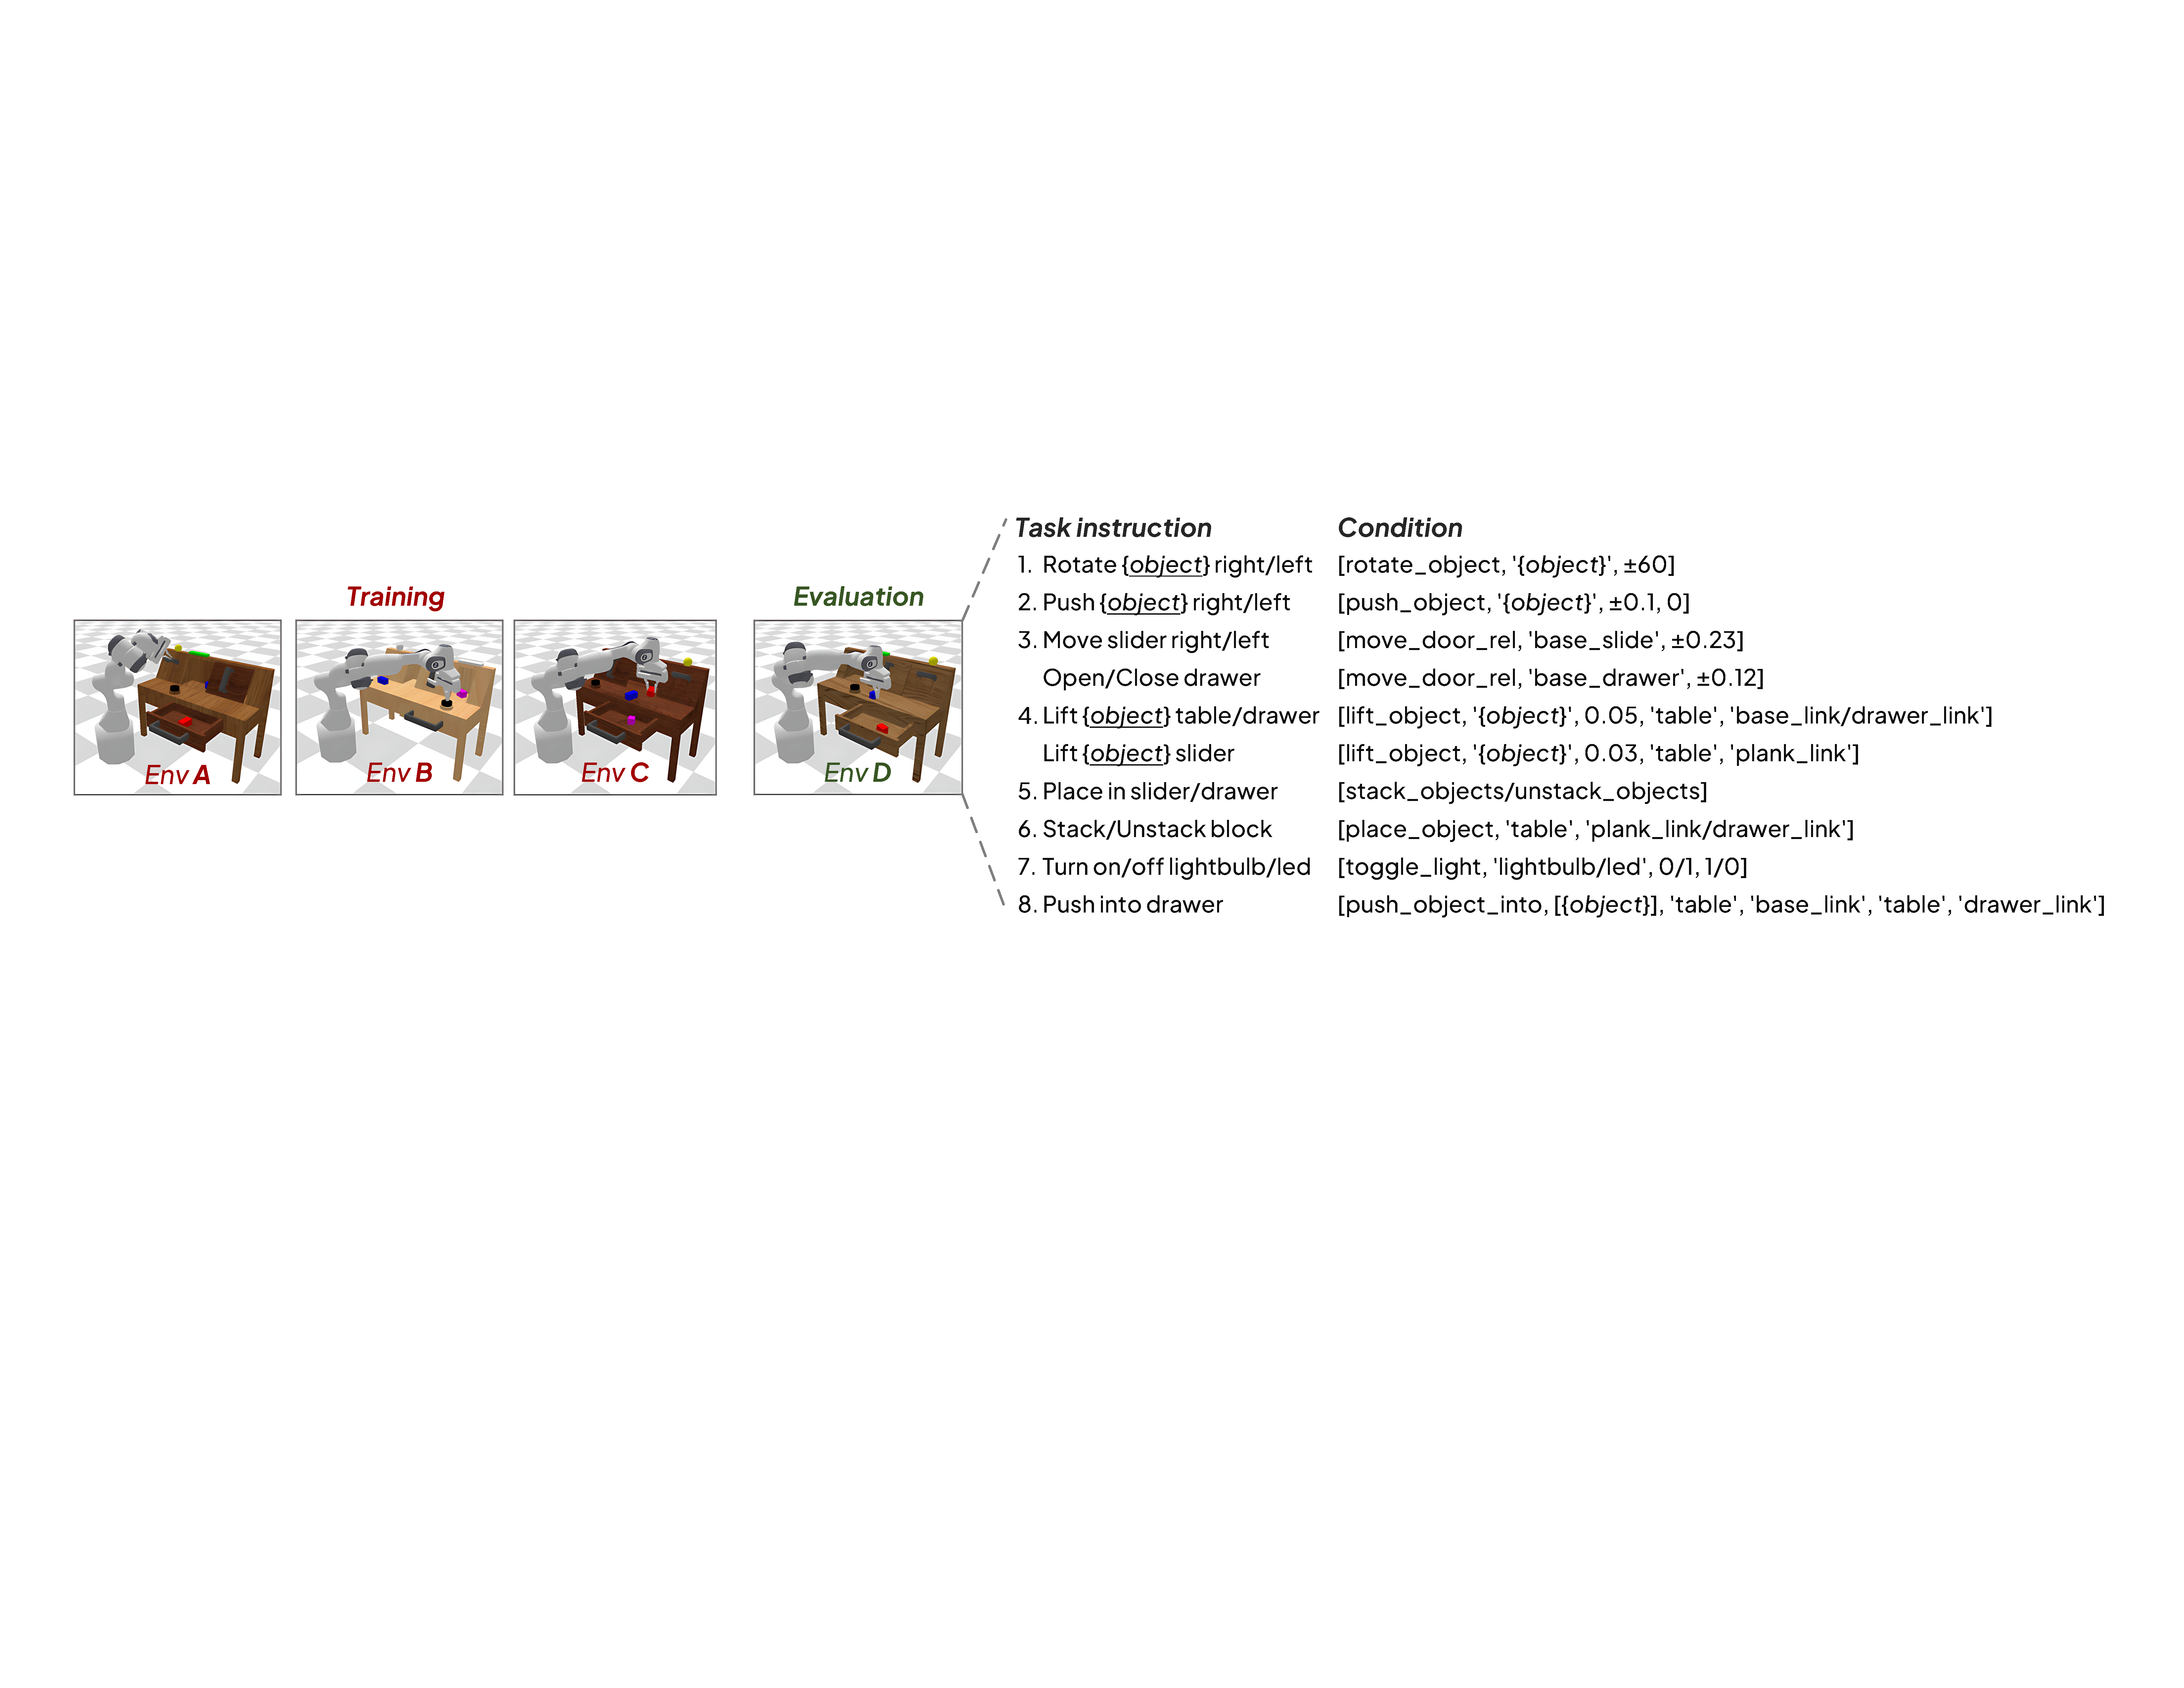
\includegraphics[width=0.99\textwidth]{Figures/Appendix-CALVIN.pdf}	
	\caption{The example and task completion conditions on the CALVIN ABC$\to$D.}\label{Figure_CALVIN_Bench}
\end{figure}

In the CALVIN ABC$\to$D benchmark, we use third-person images (resolution 224$\times$224$\times$3, RGB) and Gripper images (resolution 84$\times$84$\times$3, RGB) as visual input. The task instruction is first constructed as a prompt in a specific format: ``\texttt{In: What action should the robot take to \{Task instruction\}?\textbackslash nOut:}", and then input into the VLM module together with the image information. Its output is a 7-dimensional action vector, which is used to control the 7-DOF Franka Emika Panda simulated robot arm to perform the corresponding action sequence.

\vspace{5ex}
\section{Supplementary Details of Training and Hyperparameters}\label{AppendixE}
\renewcommand{\thefigure}{F\arabic{figure}}
\renewcommand{\theHfigure}{F\arabic{figure}}
\setcounter{figure}{0}

\renewcommand{\thetable}{F\arabic{table}}
\renewcommand{\theHtable}{F\arabic{table}}
\setcounter{table}{0}

\subsection{Training Details}\label{AppendixE1}
During VLA-Adapter training, we use the AdamW \citep{AdamW-2019} optimizer and LoRA scheme \citep{LoRA-2022}. To ensure the stability of training, the learning rate is set to 1e-4, and the cosine-annealing scheduler with warm-up steps is used. Our batch size is set to 16.

\begin{table}[!htbp]
	\centering
	\caption{The detail settings of Training.}\label{TableE1}%
	\begin{tabular}{c|c}
		\toprule[1pt]
		Setting & value \\
		\midrule[0.5pt]  
            Batch size & 16 \\
		Max training step & 150,000 \\
		Learning rate & 1e-4 \\
		Warmup step & 10\% \\
		\bottomrule[1pt]
	\end{tabular}%
\end{table}%

\FloatBarrier
\subsection{Hyperparameter Details}\label{AppendixE2}
We list the hyperparameters of VLA-Adapter. Their corresponding values are shown in Table \ref{TableE2}.

\begin{table}[!htbp]
	\centering
	\caption{Specific hyperparameters of VLA-Adapter and their corresponding values.}\label{TableE2}%
	\begin{tabular}{c|c}
		\toprule[1pt]
		Backbone & Qwen2.5-0.5B\\
		Layer ($\tau$ / $M$) & 24  \\
		Number of ActionQuery & 64  \\
		Hidden size & 896   \\
		Attention head & 8      \\
		Action chunk ($H$) & 8\\
		Intermediate layers of VLM & 1--24\\
		\midrule[0.5pt]
		Total trainable parameters of Policy  &97.3M\\
            Total trainable parameters of VLA-Adapter    &197.2M\\
		\bottomrule[1pt]
	\end{tabular}%
\end{table}%

\FloatBarrier
\section{Execution Examples}\label{AppendixF}
\renewcommand{\thefigure}{G\arabic{figure}}
\renewcommand{\theHfigure}{G\arabic{figure}}
\setcounter{figure}{0}

\renewcommand{\thetable}{G\arabic{table}}
\renewcommand{\theHtable}{G\arabic{table}}
\setcounter{table}{0}

We provide some execution examples, please see Figure \ref{FigF1} and Figure \ref{FigF2} for details. 

\subsection{Real-World Examples}\label{AppendixF1}

These include long-horizon tasks: ``Pick up the spoon and place it on the cup, then place the cup on the plate" and short-horizon tasks: ``Stack red blocks on top of blue blocks", ``Move the blue block to the right", and ``Pick up the duck and place it on a plate". The settings of real-world experiments are shown in Section \ref{sec44}.

\begin{figure}[!htbp]
	\centering
	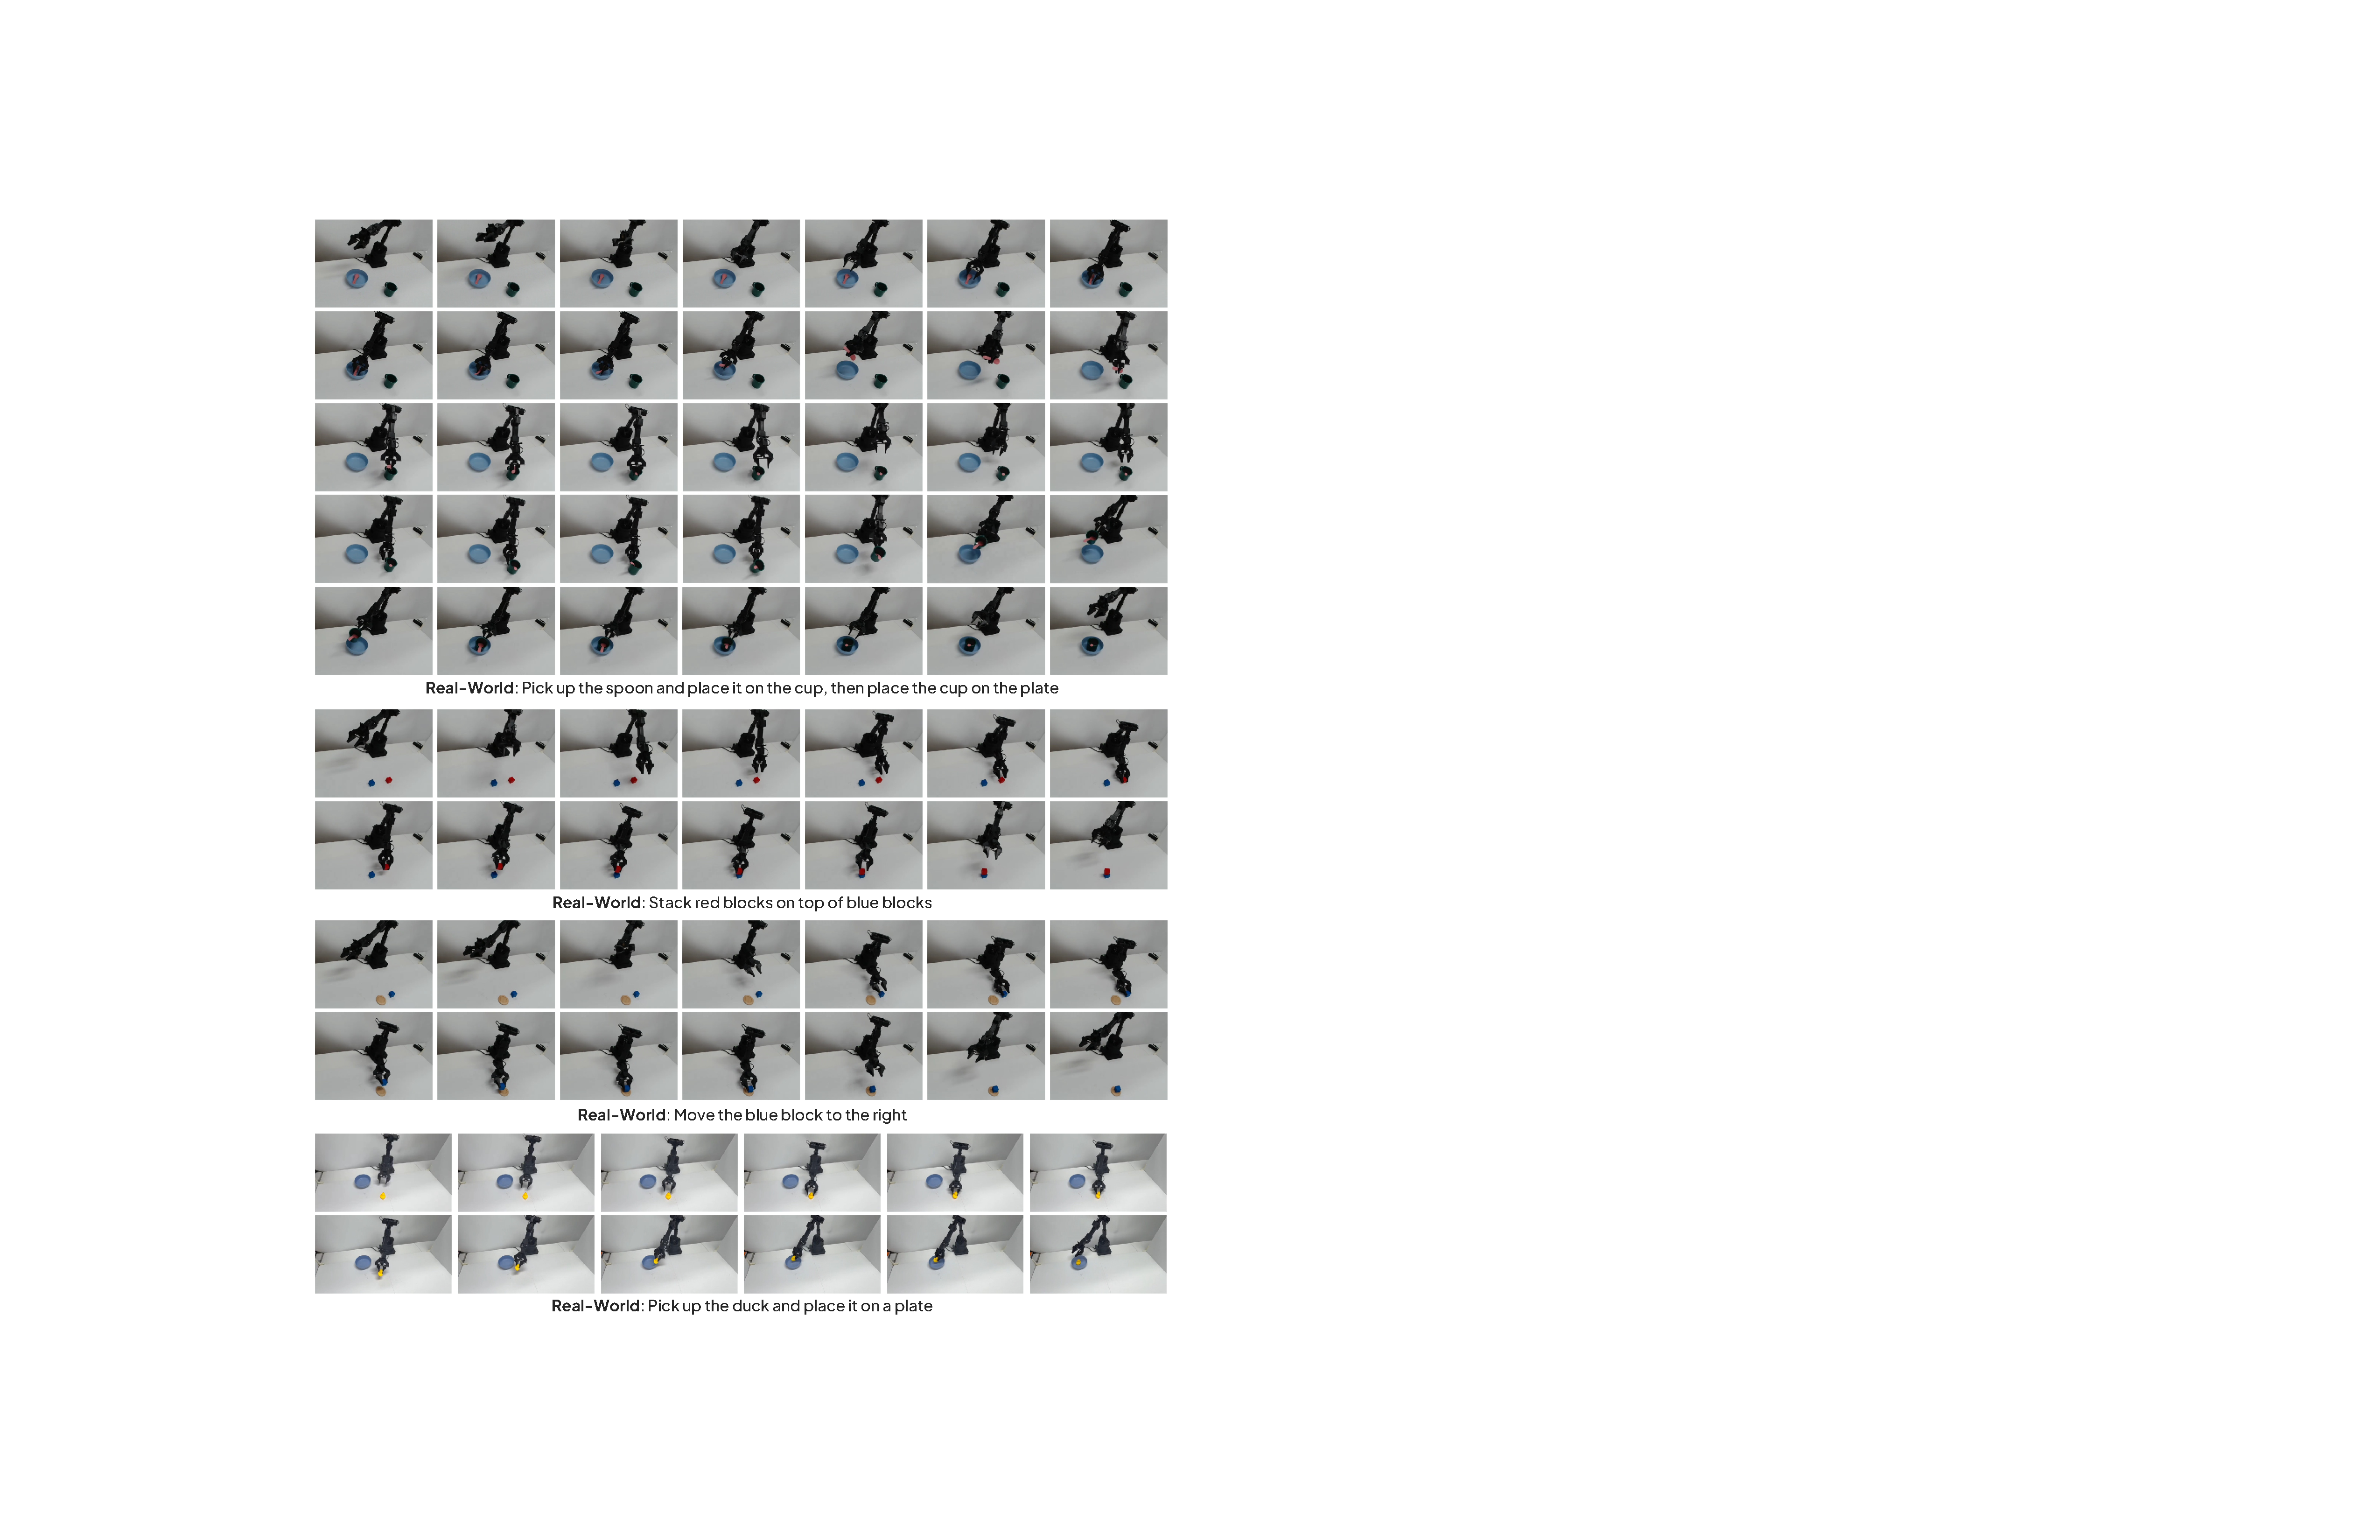
\includegraphics[width=0.99\textwidth]{Figures/realworld-example.pdf}	
	\caption{Execution example on the real-world tasks.}\label{FigF1}
\end{figure}

\FloatBarrier

\newpage
\subsection{Simulation Examples}\label{AppendixF2}

\begin{figure}[!htbp]
	\centering
	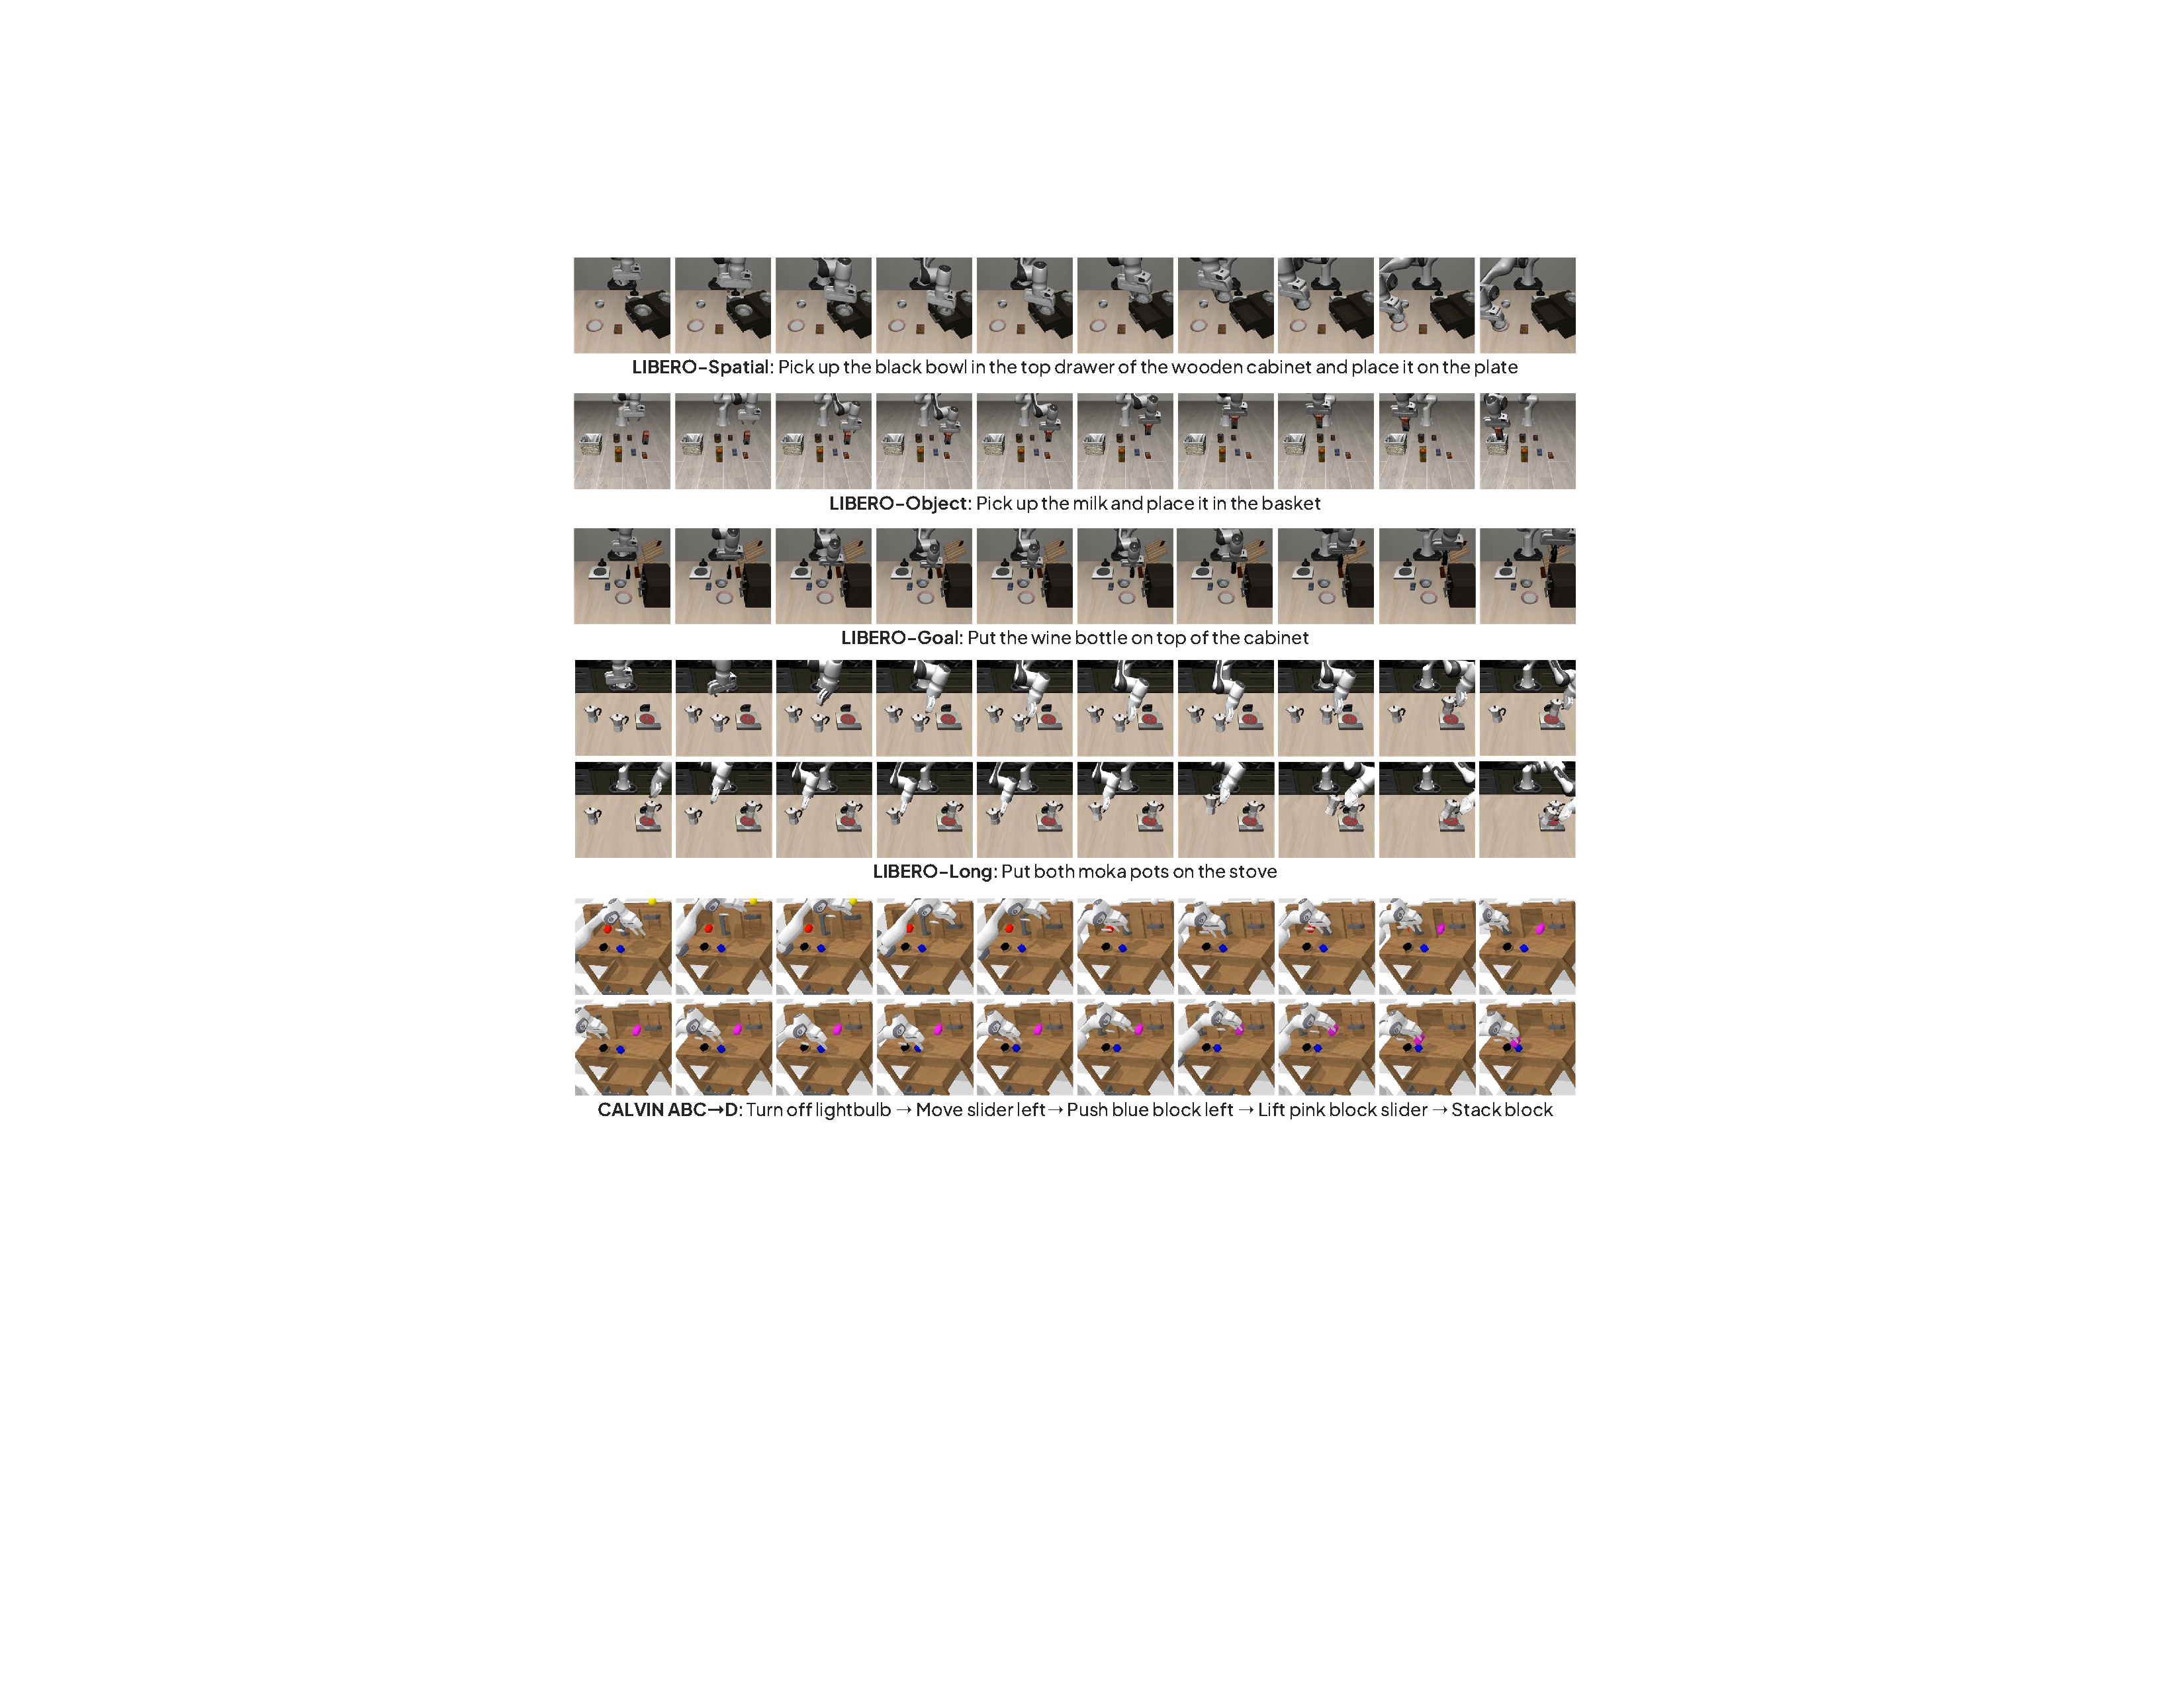
\includegraphics[width=0.99\textwidth]{Figures/CALVIN_example.pdf}	
	\caption{Execution example on the LIBERO and CALVIN ABC$\to$D tasks.}\label{FigF2}
\end{figure}

\FloatBarrier

\section{Effectiveness Analysis of Frozen Backbone}\label{AppendixG}
\renewcommand{\thefigure}{H\arabic{figure}}
\renewcommand{\theHfigure}{H\arabic{figure}}
\setcounter{figure}{0}

\renewcommand{\thetable}{H\arabic{table}}
\renewcommand{\theHtable}{H\arabic{table}}
\setcounter{table}{0}

Section \ref{sec41} compares the effectiveness of the frozen backbone. The results show that OpenVLA-OFT does not work. Although it also uses learnable tokens, it is implemented (line 620 in \footnote{\url{https://github.com/moojink/openvla-oft/blob/main/prismatic/extern/hf/modeling_prismatic.py}}):

{\small
	\begin{verbatim}
	# === Handle Multimodal Forward ===
	elif (input_ids.shape[0] == pixel_values.shape[0]) or (inputs_embeds.shape[0] 
                          == pixel_values.shape[0]):
    ...
    # Process action embeddings
    if noisy_actions is not None:
        ...
    else:
        # Replace the embeddings of the action tokens with zeros
        # (Later on, the positional embeddings will be added to them)
        all_actions_mask = all_actions_mask.unsqueeze(-1) 
        input_embeddings = input_embeddings * ~all_actions_mask
	\end{verbatim}
}

The tokens added in the ``else:" (L1 architecture) are input to the VLM in the form of a mask. It is initially all zeros, and when the VLM backbone is frozen, it is not trained. Our ActionQuery is:

{\small
	\begin{verbatim}
	# === Handle Multimodal Forward ===
	elif (input_ids.shape[0] == pixel_values.shape[0]) or (inputs_embeds.shape[0] 
                          == pixel_values.shape[0]):
    ...
    # Process action embeddings
    if noisy_actions is not None:
        ...
    else:
        action_queries = self.action_queries.weight  # (1, h)
        action_queries = action_queries.view(1, action_queries.shape[0], 
            action_queries.shape[1]).repeat(input_embeddings.shape[0], 1, 1)
                  
        all_actions_mask = self._process_action_masks(labels)
        input_embeddings = self._replace_input_embeddings(input_embeddings, 
                                                          all_actions_mask, 
                                                          action_queries)
	\end{verbatim}
}

Instead of inputting the VLM in the form of a mask, essentially learnable tokens (or multiple tokens) that is inserted into the specified position in the sequence and participate in attention. Therefore, when the VLM is frozen, the VL information is indeed not trained. Still, ActionQuery is not an original part of the VLM, and its parameters can be learned from scratch, so the VLA-Adapter still works. Below, we give examples of OpenVLA-OFT and VLA-Adapter, as shown in Figure \ref{FigG1}.

\begin{figure}[!htbp]
	\centering
	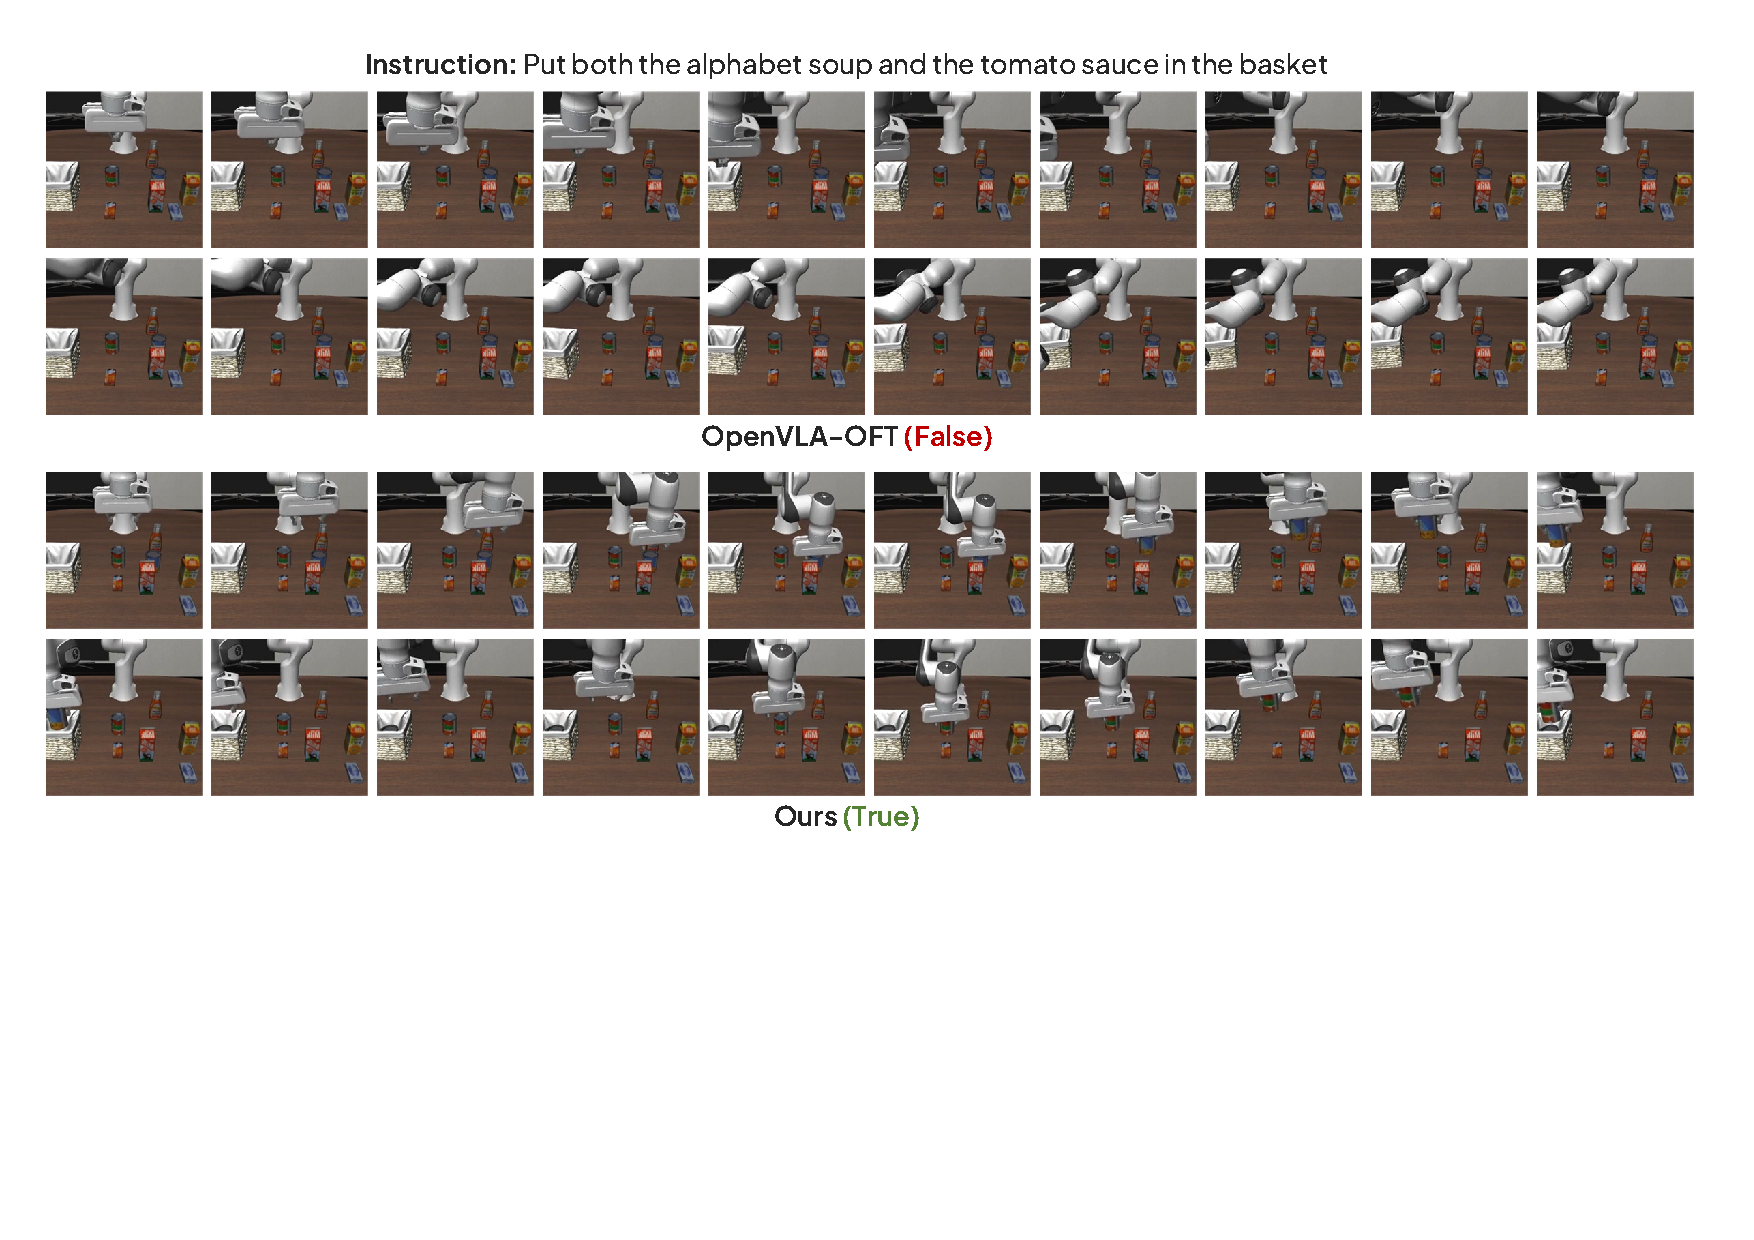
\includegraphics[width=0.99\textwidth]{Figures/False_True.pdf}	
	\caption{Execution example when the backbone is frozen.}\label{FigG1}
\end{figure}

\vspace{11ex}

\section{Design Details and Performance of VLA-Adapter-Pro}\label{AppendixI}
\renewcommand{\thefigure}{I\arabic{figure}}
\renewcommand{\theHfigure}{I\arabic{figure}}
\setcounter{figure}{0}

\renewcommand{\thetable}{I\arabic{table}}
\renewcommand{\theHtable}{I\arabic{table}}
\setcounter{table}{0}

To achieve extreme lightweightness in VLA-Adapter, we shared the projection layer, using the same projection layer for all three attention matrices. This resulted in a low parameter count of 97MB. 

In the VLA-Adapter-Pro version, we separated the projection layers for the three attention matrices, allowing different channels to learn differentiated representations. In this case, the parameter count was 207MB. Furthermore, VLA-Adapter-Pro adds Rotary Position Embedding to QK, making the cross-attention more sensitive to position information and more suitable for action generation.

Next, we give the key architecture codes of VLA-Adapter-Pro, as shown below:

{\small
\begin{verbatim}
class MLPResNetBlock_Pro(nn.Module):
    """One MLP ResNet block with 
    separate projections for self, adapter, task 
    + 
    RoPE, now without FiLM modulation."""

    def __init__(self, dim, num_heads=8):
        super().__init__()
        self.dim = dim
        self.num_heads = num_heads
        self.head_dim = dim // num_heads

        self.ffn = nn.Sequential(
            nn.LayerNorm(dim),
            nn.Linear(dim, dim),
            nn.ReLU(),
            )

        # Q (from x only)
        self.q_proj = nn.Linear(dim, dim)

        # Self-Attention: K, V
        self.k_self = nn.Linear(dim, dim)
        self.v_self = nn.Linear(dim, dim)

        # Adapter cross-attention: K, V
        self.k_adapter = nn.Linear(dim, dim)
        self.v_adapter = nn.Linear(dim, dim)

        # Task cross-attention: K, V
        self.k_task = nn.Linear(dim, dim)
        self.v_task = nn.Linear(dim, dim)

        self.o_proj = nn.Linear(dim, dim)

        # gating
        self.gating_factor = nn.Parameter(torch.zeros(1))

        # RoPE
        self.rope = RotaryPositionEmbedding(self.head_dim)

        # ---- FiLM ----
        # # FiLM is useless; to avoid conflict with chkpt, it can be kept as is for now.
        self.film_gen = nn.Sequential(
            nn.Linear(dim, dim * 2), 
            )


    def apply_film(self, x, gamma, beta):
        """FiLM: per-channel modulation"""
        return gamma.unsqueeze(1) * x + beta.unsqueeze(1)


    def forward(self, x, h_a=None, h_t=None, p=None):
        """
        h_a: adapter tokens
        h_t: task tokens
        p:   possible conditioning vector (for FiLM)
        """
        g = self.gating_factor
        ratio_g = torch.tanh(g)

        # concat h_a and p
        h_adapter = torch.cat((h_a, p),dim=1)

        h_task = h_t
        B, T, C = x.shape
        K_a = h_adapter.size(1) if h_a is not None else 0
        K_t = h_task.size(1) if h_task is not None else 0

        # Q
        q_1 = self.q_proj(x)

        # self tokens
        k_tokens = self.k_self(x)
        v_tokens = self.v_self(x)

        # adapter tokens
        k_adapter = self.k_adapter(h_adapter)
        v_adapter = self.v_adapter(h_adapter)

        # task tokens
        k_task = self.k_task(h_task)
        v_task = self.v_task(h_task)


        # reshape -> multi-head
        def reshape_heads(t, B, L):
            return t.view(B, L, self.num_heads, self.head_dim).transpose(1, 2)


        q_1 = reshape_heads(q_1, B, T)
        k_tokens, v_tokens = reshape_heads(k_tokens, B, T), reshape_heads(v_tokens, B, T)
        k_adapter, v_adapter = reshape_heads(k_adapter, B, K_a), reshape_heads(v_adapter, B, K_a)
        k_task, v_task = reshape_heads(k_task, B, K_t), reshape_heads(v_task, B, K_t)

        # RoPE
        cos_main, sin_main = self.rope(seq_len=T, device=x.device, dtype=x.dtype)
        q_1, k_tokens = apply_rope(q_1, k_tokens, cos_main, sin_main)
        cos_a, sin_a = self.rope(seq_len=K_a, device=x.device, dtype=x.dtype)
        _, k_adapter = apply_rope(k_adapter, k_adapter, cos_a, sin_a)     
        cos_t, sin_t = self.rope(seq_len=K_t, device=x.device, dtype=x.dtype)
        _, k_task = apply_rope(k_task, k_task, cos_t, sin_t)

        # attention scores
        attn_scores = [torch.matmul(q_1, k_tokens.transpose(-2, -1))]
        attn_scores.append(torch.matmul(q_1, k_adapter.transpose(-2, -1)))
        attn_scores.append(torch.matmul(q_1, k_task.transpose(-2, -1)) * ratio_g)
        attn_scores = torch.cat(attn_scores, dim=-1) / math.sqrt(self.head_dim)
        attn_weights = torch.softmax(attn_scores, dim=-1)

        # combine V
        v_list = [v_tokens,v_adapter,v_task]
        v_combined = torch.cat(v_list, dim=2)

        output = torch.matmul(attn_weights, v_combined)
        output = output.transpose(1, 2).contiguous().view(B, T, C)
        output = self.o_proj(output)

        # # ---- FiLM ---- 
        # gamma_beta = self.film_gen(p)  # [B, 2C]
        # gamma, beta = gamma_beta.chunk(2, dim=-1)  # [B, C], [B, C]
        # output = self.apply_film(output, gamma, beta)

        # residual + FFN
        x = self.ffn(output + x)
        return x

\end{verbatim}
}

We also present the performance comparison between VLA-Adapter and VLA-Adapter-Pro on 40 subtasks on LIBERO, as shown in Table \ref{TableI1}.

\begin{table}[!htbp]
	\centering
    \setlength{\tabcolsep}{1mm}
	\caption{The specific performance of VLA-Adapter and VLA-Adapter-Pro on the 40 subtasks of four LIBERO \citep{LIBERO-2023} suites.}\label{TableI1}%
	\begin{tabular}{c|cccccccccc|c}
		\toprule[1pt]
		Spatial & 1     & 2     & 3     & 4     & 5     & 6     & 7     & 8     & 9     & 10    & \textbf{Avg. $\uparrow$} \\
		\midrule[0.5pt]
		VLA-Adapter &  98.0     &   \textbf{100.0}    &   100.0    & 90.0      &   96.0    &  100.0     &   100.0    &    100.0   &    98.0   &    96.0   & 97.8 \\
        VLA-Adapter-Pro &  \textbf{100.0}     &   98.0    &   100.0    & \textbf{100.0}      &   \textbf{100.0}    &  100.0     &   100.0    &    100.0   &    \textbf{100.0}   &    \textbf{98.0}   & \textbf{99.6} \\
        \midrule[1pt]
        
		Object & 1     & 2     & 3     & 4     & 5     & 6     & 7     & 8     & 9     & 10    & \textbf{Avg. $\uparrow$} \\
		\midrule[0.5pt]
        VLA-Adapter & 98.0  & 98.0  & 100.0  & 100.0  & 98.0  & 100.0 & 98.0  & 100.0 & 100.0  & 100.0 & 99.2 \\
        VLA-Adapter-Pro & \textbf{100.0}  & \textbf{100.0}  & 100.0  & 100.0  & 98.0  & 100.0 & 98.0  & 100.0 & 100.0  & 100.0 & \textbf{99.6} \\
        \midrule[1pt]
        
		Goal & 1     & 2     & 3     & 4     & 5     & 6     & 7     & 8     & 9     & 10    & \textbf{Avg. $\uparrow$} \\
        \midrule[0.5pt]
        VLA-Adapter&   92.0    &    100.0   &   \textbf{98.0}    &    96.0   &     100.0  &    98.0   &   94.0    &   100.0    &  98.0     &   96.0    & 97.2 \\
        VLA-Adapter-Pro & \textbf{98.0}  &100.0  & 94.0  & 96.0  & 100.0  & 98.0 & \textbf{96.0}  & 100.0 &\textbf{100.0}  & \textbf{100.0} & \textbf{98.2} \\
        \midrule[1pt]
        
		Long  & 1     & 2     & 3     & 4     & 5     & 6     & 7     & 8     & 9     & 10    & \textbf{Avg. $\uparrow$} \\
        \midrule[0.5pt]
        VLA-Adapter&\textbf{96.0}&96.0& \textbf{100.0} &\textbf{98.0}&\textbf{100.0}&100.0& 84.0& 96.0& 84.0& 96.0&95.0 \\
        VLA-Adapter-Pro&92.0&\textbf{100.0}& 98.0 &96.0&94.0&100.0& \textbf{94.0}& \textbf{100.0}& \textbf{90.0}& \textbf{100.0}&\textbf{96.4} \\
		\bottomrule[1pt]
	\end{tabular}%
\end{table}%